%%%%%%%%%%%%%%%%%%%%%%%%%%%%%%%%%%%%%%%%%
% baposter Landscape Poster
% LaTeX Template
% Version 1.0 (11/06/13)
%
% baposter Class Created by:
% Brian Amberg (baposter@brian-amberg.de)
%
% This template has been downloaded from:
% http://www.LaTeXTemplates.com
%
% License:
% CC BY-NC-SA 3.0 (http://creativecommons.org/licenses/by-nc-sa/3.0/)
%
%%%%%%%%%%%%%%%%%%%%%%%%%%%%%%%%%%%%%%%%%

%----------------------------------------------------------------------------------------
%	PACKAGES AND OTHER DOCUMENT CONFIGURATIONS
%----------------------------------------------------------------------------------------

\documentclass[landscape,a0paper,fontscale=0.285]{baposter} % Adjust the font scale/size here
% Initial size : 0.285
\usepackage{graphicx} % Required for including images
\graphicspath{{figures/}} % Directory in which figures are stored

\usepackage{pgf}
\usepackage{tcolorbox}
\usepackage{amsmath} % For typesetting math
\usepackage{amssymb} % Adds new symbols to be used in math mode
\usepackage{mathrsfs}
%\usepackage{mathtools}

\usepackage{caption} 




\usepackage{url}

\usepackage{booktabs} % Top and bottom rules for tables
\usepackage{enumitem} % Used to reduce itemize/enumerate spacing
\usepackage{palatino} % Use the Palatino font
\usepackage[font=small,labelfont=bf]{caption} % Required for specifying captions to tables and figures

\usepackage{multicol} % Required for multiple columns
\setlength{\columnsep}{1.25em} % Slightly increase the space between columns
\setlength{\columnseprule}{0mm} % No horizontal rule between columns

\usepackage{tikz} % Required for flow chart
\usetikzlibrary{shapes,arrows} % Tikz libraries required for the flow chart in the template

\newcommand{\compresslist}{ % Define a command to reduce spacing within itemize/enumerate environments, this is used right after \begin{itemize} or \begin{enumerate}
\setlength{\itemsep}{1pt}
\setlength{\parskip}{0pt}
\setlength{\parsep}{0pt}
}

\definecolor{bleutitre}{rgb}{0,0,1}
\definecolor{f1}{rgb}{0.7,0,0}
\definecolor{f2}{rgb}{0,0.7,0}
\definecolor{f3}{rgb}{0,0,0.7}
\newcommand{\fa}{{\color{f1}f_1}}
\newcommand{\fb}{{\color{f2}f_2}}
\newcommand{\fc}{{\color{f3}f_3}}


\newlist{citemize}{itemize}{1}
\setlist[citemize]{label=\textcolor{bleutitre}{\textbullet}}






\newcommand{\dataset}{\ensuremath{\mathcal{D}}}
\newcommand{\loss}{\ensuremath{\mathcal{L}}}
\newcommand{\ntrain}{\ensuremath{N}}
\newcommand{\R}{\ensuremath{\mathbb{R}}}
\newcommand{\x}{\ensuremath{\mathbf{x}}} % predicted and general x
\newcommand{\tx}{\ensuremath{\tilde{\mathbf{x}}}} % training x 
\newcommand{\eps}{\ensuremath{\epsilon}}

\newcommand{\params}{\ensuremath{\boldsymbol{\theta}}}
\newcommand{\nnet}{\ensuremath{f_{\params}}}



\begin{document}

\begin{poster}
{
headerborder=closed, % Adds a border around the header of content boxes
colspacing=1em, % Column spacing
bgColorOne=white, % Background color for the gradient on the left side of the poster
bgColorTwo=white, % Background color for the gradient on the right side of the poster
borderColor=black, % Border color
headerColorTwo=white, % Background color for the header in the content boxes (left side)
headerColorOne=white, % Background color for the header in the content boxes (right side)
headerFontColor=black, % Text color for the header text in the content boxes
boxColorOne=white, % Background color of the content boxes
textborder=bars, % Format of the border around content boxes, can be: none, bars, coils, triangles, rectangle, rounded, roundedsmall, roundedright or faded
eyecatcher=true, % Set to false for ignoring the left logo in the title and move the title left
headerheight=0.2\textheight, % Height of the header
headershape=smallrounded, % Specify the rounded corner in the content box headers, can be: rectangle, small-rounded, roundedright, roundedleft or rounded
headerfont=\Large\bf\textsc, % Large, bold and sans serif font in the headers of content boxes
%textfont={\setlength{\parindent}{1.5em}}, % Uncomment for paragraph indentation
linewidth=1pt % Width of the border lines around content boxes
}
%----------------------------------------------------------------------------------------
%	TITLE SECTION 
%----------------------------------------------------------------------------------------
%
{
  \begin{minipage}{0.2\textwidth}
    
\includegraphics[height=2.5em]{dauphine}\\
    
\includegraphics[height=4.5em]{logomiles_white}\\[1ex]
    
\includegraphics[height=2.7em]{espci}%        
  \end{minipage}
}
% First university/lab logo on the left
{{\color{bleutitre}Experimental study of Neural ODE training with\\[0.5ex] adaptive solver
  for dynamical systems modeling}\vspace{1ex}} % Poster title
{  Alexandre Allauzen $^{1,2}$, Thiago Petrilli Maffei Dardis$^{2}$, Hannah Plath$^{2}$\\
  $^{1}$LAMSADE CNRS, Dauphine University-PSL, $^{2}$ESPCI-PSL
} % Author names
{} % Third logo




%%%%%%%%%%%%%%%%%%%%%%%%%%%%%%%%%%%%%%%%%%%%%%%%%%%%%%%%%%%%%%%%%%%%%%%%%%%%%%%%%%%%%%%
\headerbox{Take-home message: whatch your step size !}{headerFontColor=red,name=abstract,span=2,column=0,row=0}{
  \begin{citemize}
  \item Neural Ordinary Differential Equations (\textbf{ODE}s) relies on
     solvers for inference and training. 
  \item Some solvers can \textbf{adapt} their evaluation strategy depending on the
    complexity of the problem.
  \item By taking the Lorenz'63 system as a showcase,  a naive application
    of the Fehlberg's method does not yield the expected
    results. 
  \item  Adaptive solvers cannot be seamlessly
    leveraged as a black-box: % for dynamical systems modelling.
  \end{citemize}
  \vspace{-1.5ex}
  \begin{tcolorbox}[colback=red!5!white,colframe=red!75!black]
    \begin{citemize}
    \item[$\rightarrow$] For most of the numerical methods, the step size is adapted given the self-estimated error of the model.
    \item[$\rightarrow$] Neural ODE model is always self-confident, and the ``adaptive'' ability is under-used. 
    \item[$\rightarrow$] A simple workaround:
    \end{citemize}
    \begin{center}
      use the supervision within the solver.
    \end{center}
    \vspace{-1ex}
    \hfill\url{https://github.com/Allauzen/adaptive-step-size-neural-ode}
  \end{tcolorbox}
  ~~
}



%%%%%%%%%%%%%%%%%%%%%%%%%%%%%%%%%%%%%%%%%%%%%%%%%%%%%%%%%%%%%%%%%%%%%%%%%%%%%%%%%%%%%%%%%%%%%%%%%%%%%%
\headerbox{Neural ODE and Fehlberg's method}{headerFontColor=bleutitre,name=eq,span=2,column=2,row=0}{
  \begin{citemize}\compresslist
  \item Given $\dataset=(\tx_{i})_{i=1}^{\ntrain}$, Neural ODE learns: $\dot{\x} = \nnet (\x)$ ($\nnet$ is a NNet
    ans $\params$ its set of parameters).
  \item Inference requires a  solver: $ {\x}_{i}=\textrm{ODE\_Solve}(\nnet, \tx_i)$ and the loss function is\\[-1ex]
   $$\loss(\params, \dataset) = \sum_{i=1}^{N} ||\tilde{\x}_i - \x_i ||^2.$$
  \end{citemize}
   
   {\bf\color{bleutitre} Fehlberg's solver:} starting with a step size $h=1$, compute:
    \begin{align*}
      {\color{f1} \fa = \nnet(\x_i)},\phantom{xxxxx} 
      {\color{f2} \fb = \nnet(\x_i+h\fa)}, \phantom{xxxxx} 
      {\color{f3} \fc = \nnet(\x_i+\frac{h}{4}[\fa+\fb])}\text{ then} \phantom{xxxxx} \\
      A_1 = \x_i+\frac{h}{2}[\fa+\fb] \text{ (RK2)}  \phantom{xxx} A_2 = \x_i+\frac{h}{6}[\fa+\fb+4\fc] \text{ (RK3).} 
      \phantom{xxx}
      \rightarrow
      \phantom{xxx}
      r = \frac{|A_1-A_2|}{h} \approx Kh^2
    \end{align*}
   With the error rate $  $, then:
   \begin{citemize}\compresslist
   \item If $r > \eps=0.1$ (tolerance), $A_2$ is rejected and restart the computation with a new
     step size\\ $h'= S \times h\sqrt{\epsilon/r},\ S=0.9$ is a safety
     factor.
   \item Otherwise accept $A_2$ as ${\x}_{i+1}$
   \end{citemize}
   ~~
}

%%%%%%%%%%%%%%%%%%%%%%%%%%%%%%%%%%%%%%%%%%%%%%%%%%%%%%%%%%%%%%%%%%%%%%%%%%%%%%%%%%%%%%%
\headerbox{First round}{headerFontColor=bleutitre,name=exp1,span=2,column=0,row=0.45}{
  \vspace{-2ex}
  \begin{center}
    \hspace{-10ex}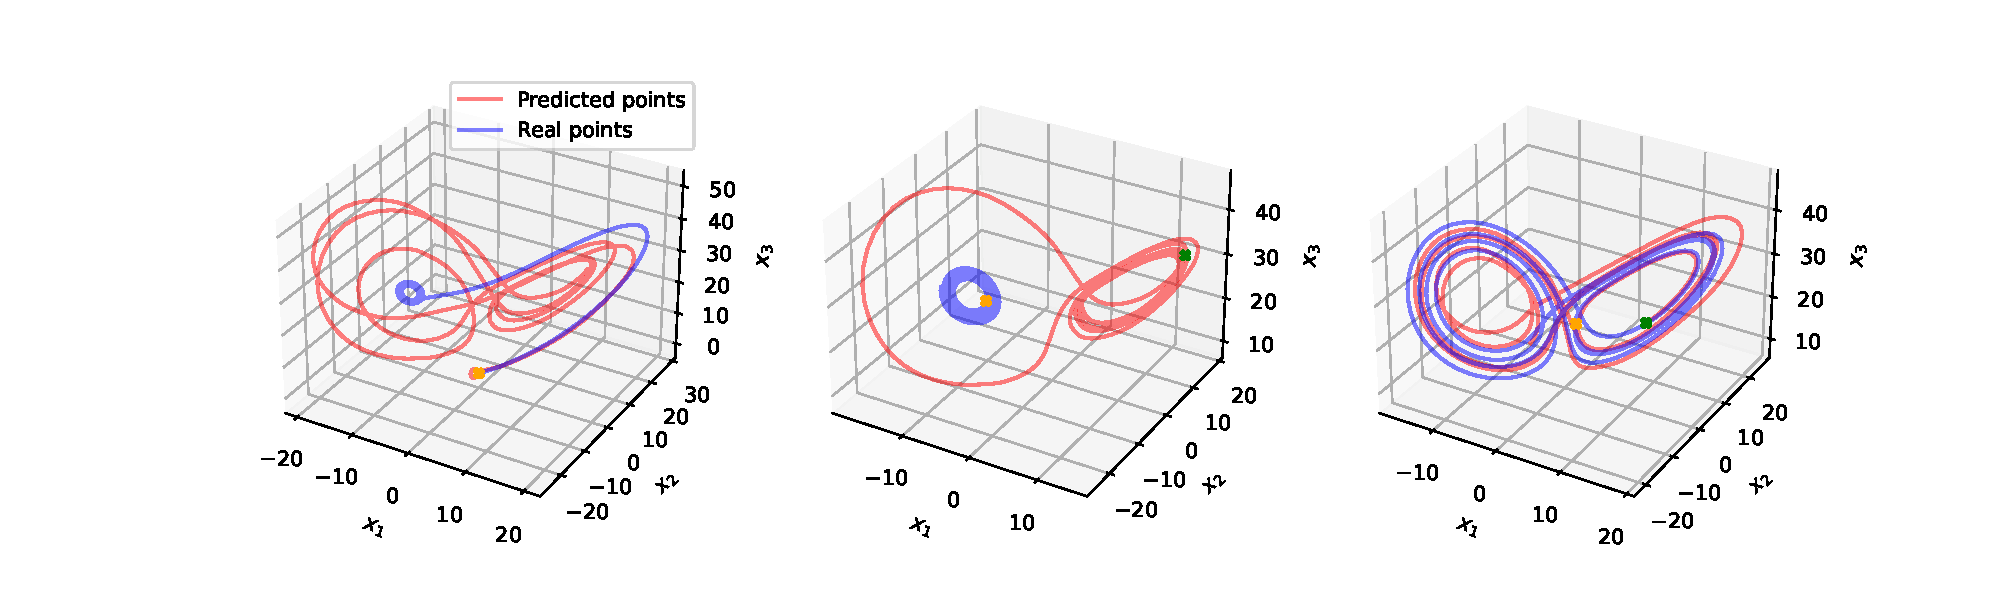
\includegraphics[width=0.8\textwidth]{../figs/baseline_lorenz_3}
    \\
    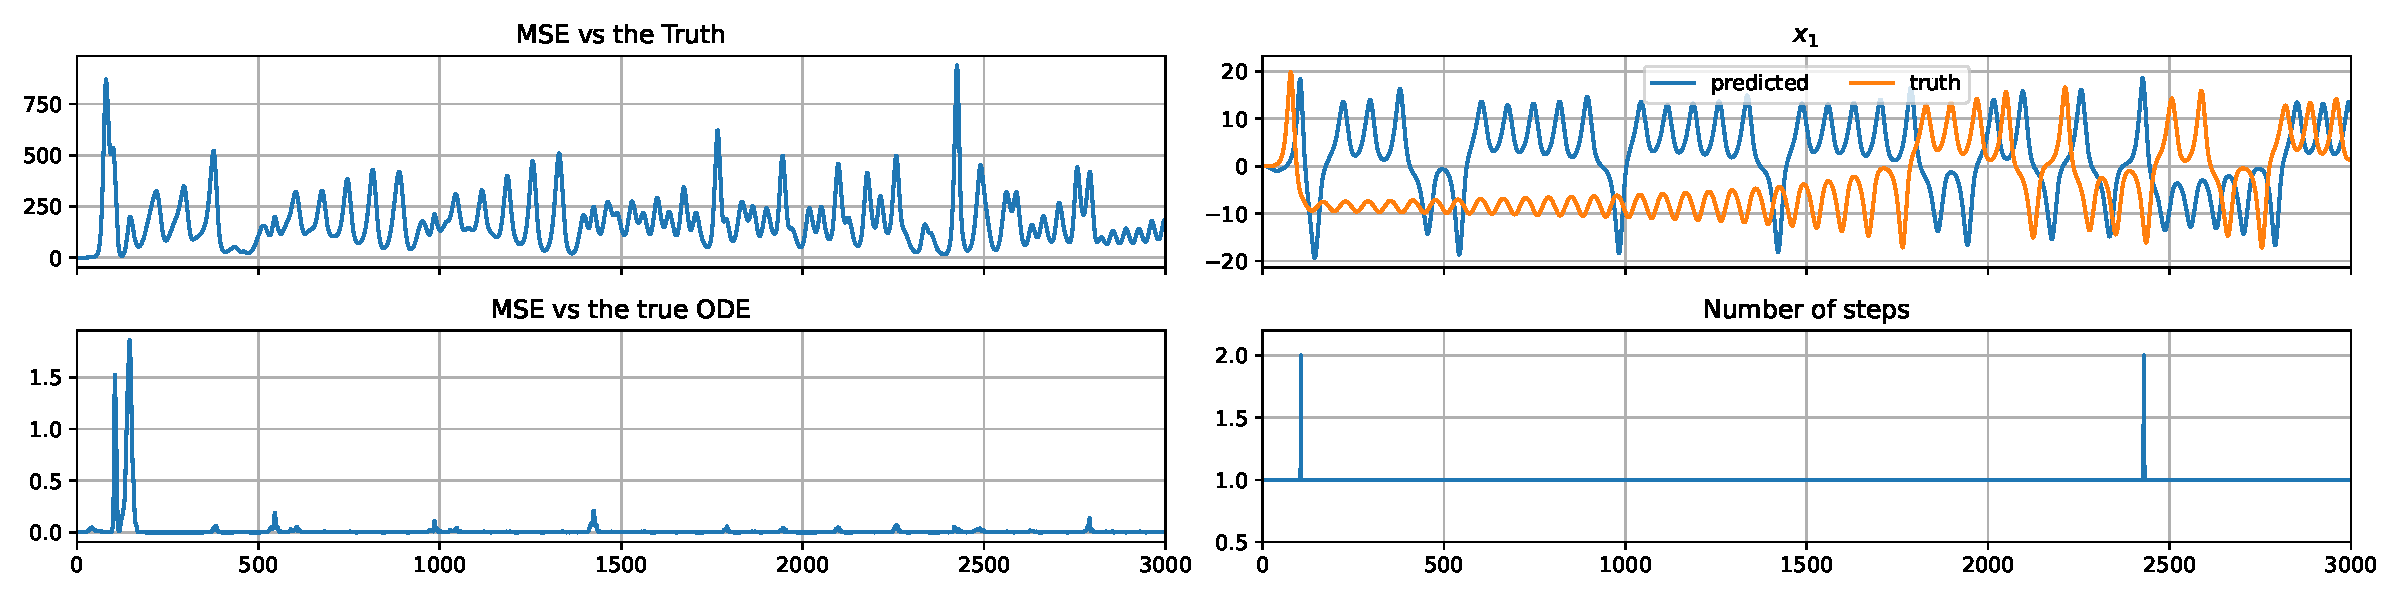
\includegraphics[width=0.8\textwidth]{../figs/baseline_time_series_2x2}
    \captionof{figure}{Time evolution of (from left to right and top to bottom):
    the MSE, the evolution of $x_1$, the MSE \textit{w.r.t} the true ODE of
    Lorenz'63, and  the number of
    steps.}
  \end{center}
}


%%%%%%%%%%%%%%%%%%%%%%%%%%%%%%%%%%%%%%%%%%%%%%%%%%%%%%%%%%%%%%%%%%%%%%%%%%%%%%%%%%%%%%%%%%%%%%%
\headerbox{Fehlberg's training}{headerFontColor=bleutitre,name=exp2,span=2,column=2,row=0.45}{
  ~\\[0.4ex]
  \begin{minipage}{1.05\textwidth}
    \begin{center}
      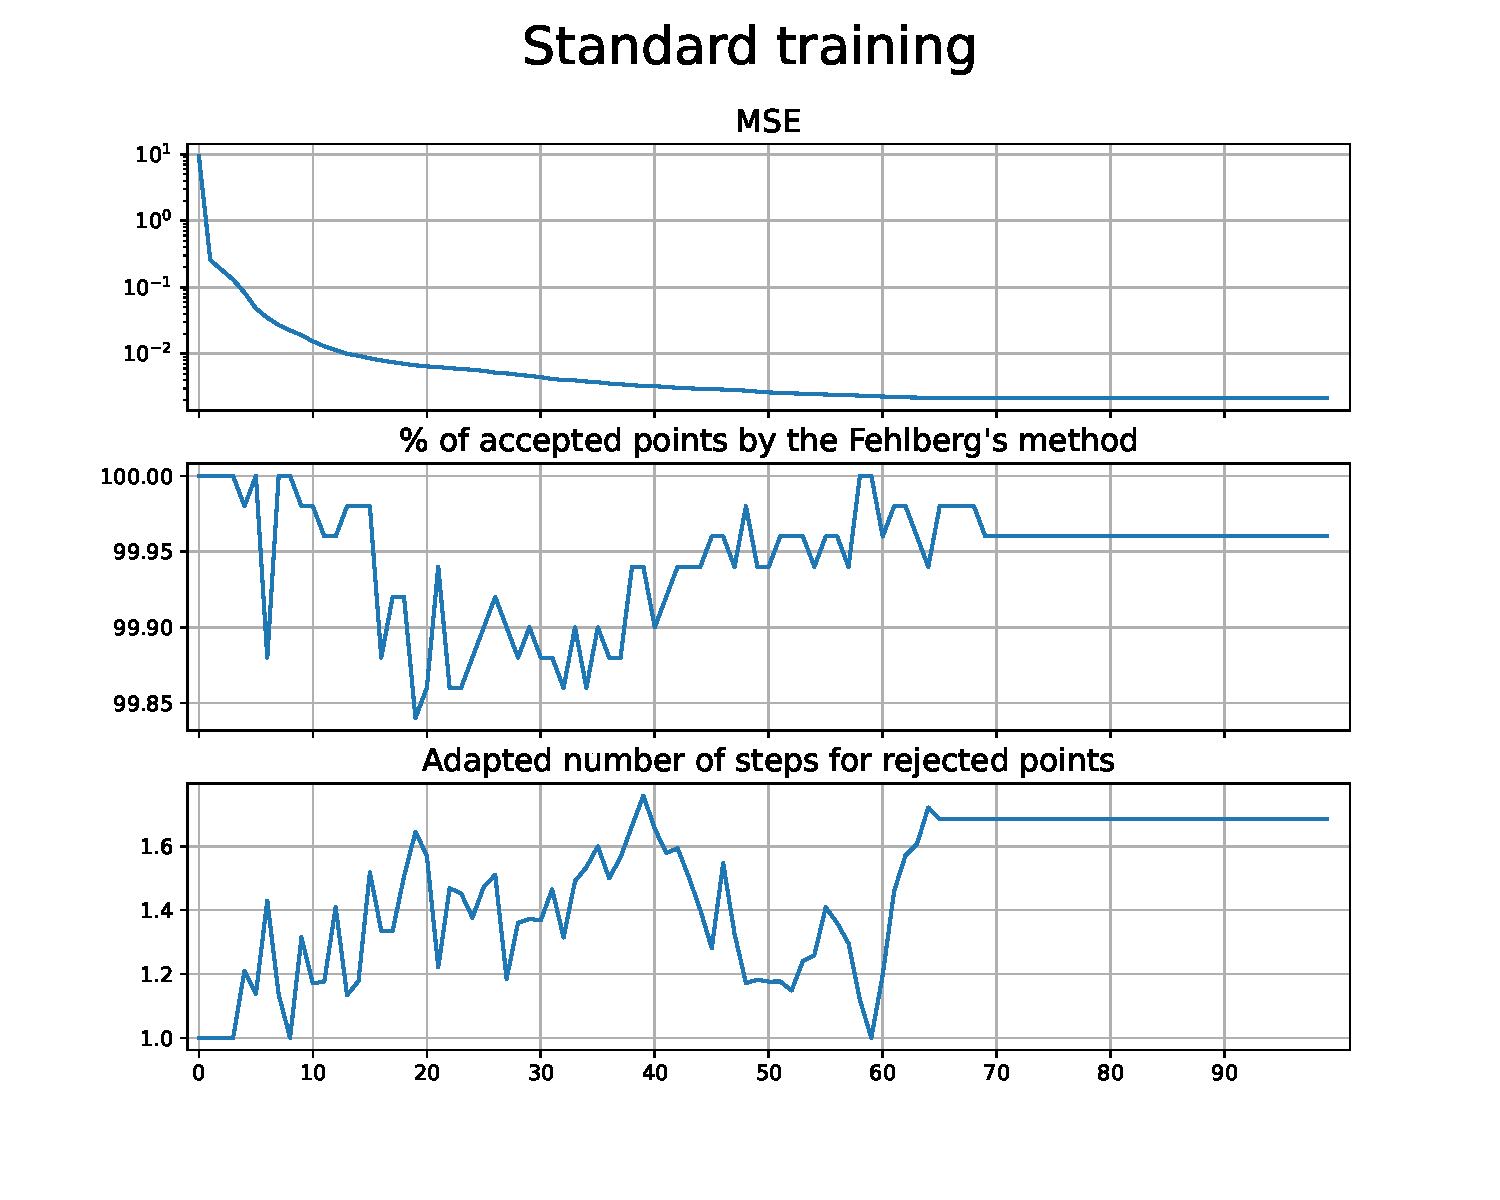
\includegraphics[width=0.49\textwidth]{../figs/batch_training}
      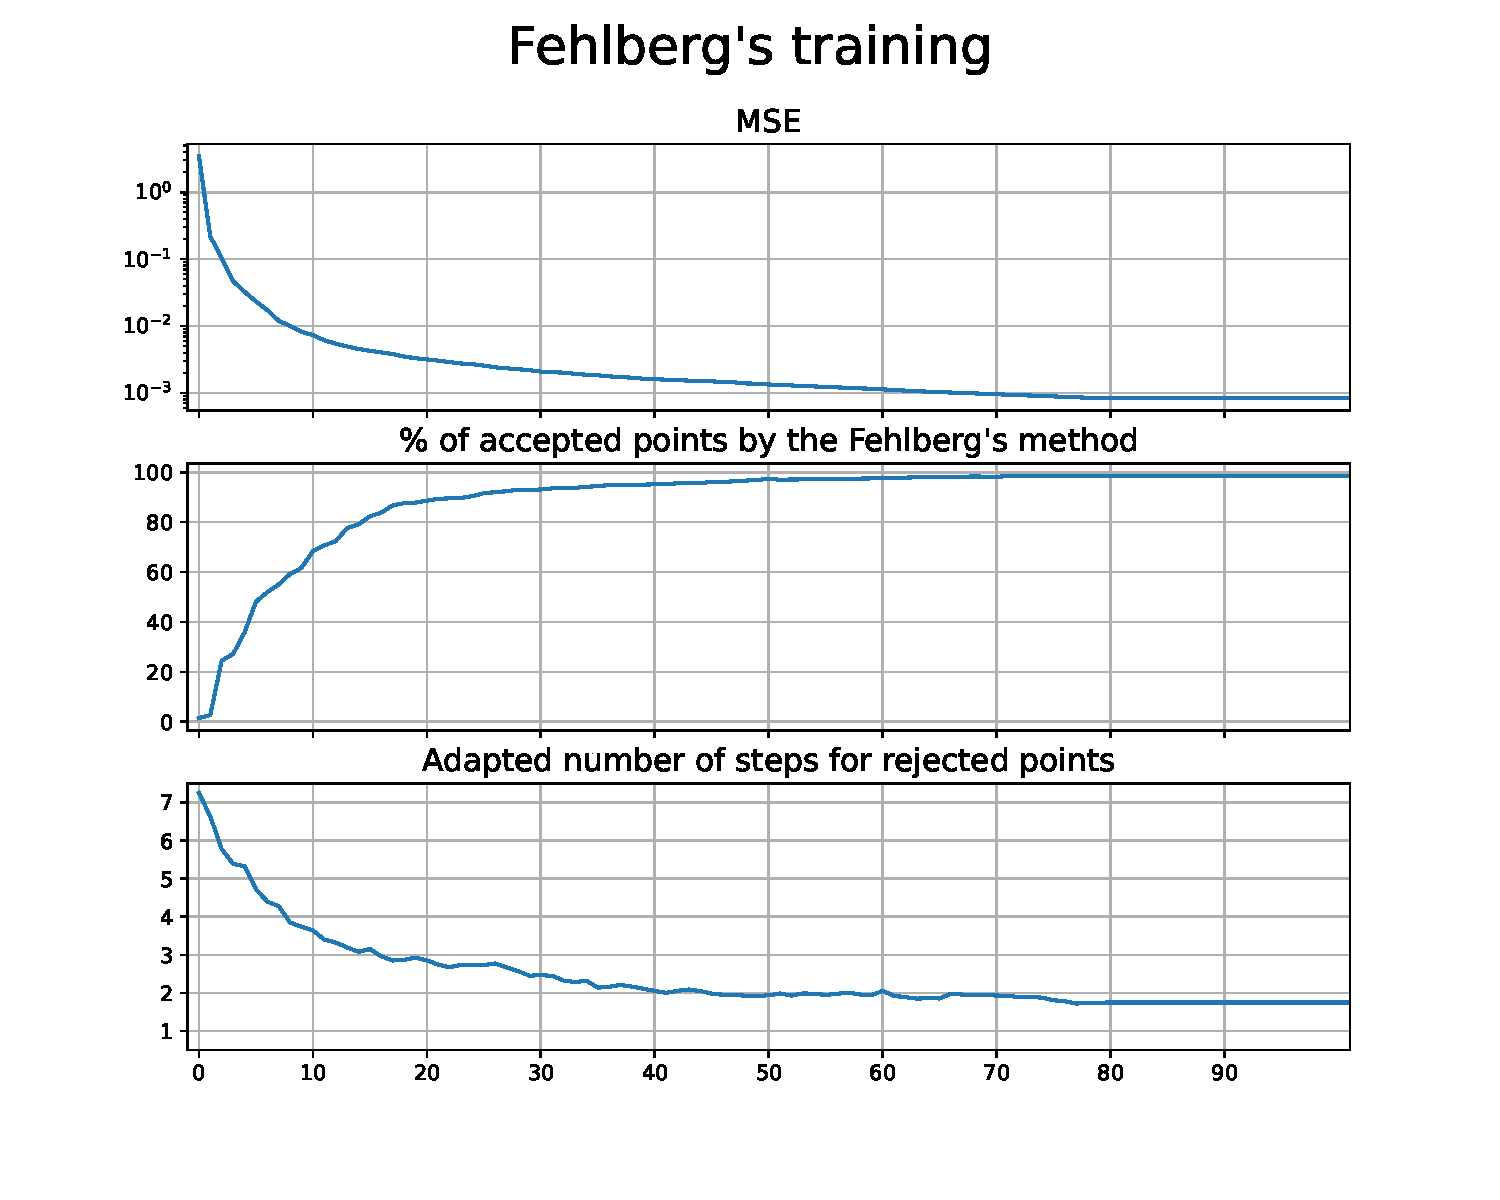
\includegraphics[width=0.49\textwidth]{../figs/fehlberg_training}\vspace{0.5ex}
    \end{center}
  \end{minipage}
  \captionof{figure}{Time evolution for two training conditions of: the MSE loss; the percentage of
    accepted hypotheses $A_2$; the new number of steps for the rejected
    hypotheses (before rounding).}
}


%----------------------------------------------------------------------------------------
%	REFERENCES or Aknowledgment
%----------------------------------------------------------------------------------------

\headerbox{Aknowledgment}{name=references,column=0,span=4,above=bottom}{
This work was funded by the French National Research Agency (SPEED-20-CE23-0025).
}


\end{poster}
\end{document}